% Screenshot helper: shows a placeholder box if the image file is missing
\providecommand{\rolefivefig}[3]{% #1 = image path, #2 = width, #3 = placeholder text
  \IfFileExists{#1}{\includegraphics[width=#2]{#1}}%
  {\fbox{\parbox{0.8\textwidth}{\centering\vspace{1.2cm}[Insert screenshot: #3]\vspace{1.2cm}}}}}

\chapter{Concurrency Control, Lock Manager Internals, Deadlock Resolution, and MVCC (Role 5)}
\label{chap:concurrency-control}

This chapter provides a comprehensive evaluation of concurrency control in Microsoft SQL Server across the clinical lumbar spine MRI workload (575 patients, 48,345 scans, 48,345 feature vectors). It integrates two complementary paradigms:
\begin{enumerate}[label=(\roman*)]
  \item \textbf{Pessimistic Concurrency Control:} Investigates Two-Phase Locking (Strict 2PL, Rigorous 2PL), internal Lock Manager architecture, lock granularity hierarchies, operational lock modes, Key-Range locking under \code{SERIALIZABLE}, and Lock Escalation dynamics across Canonical Queries Q1, Q2, and Q3.
  \item \textbf{Deadlock Resolution and Multi-Version Concurrency Control:} Evaluates automated cycle detection via the SQL Server Lock Monitor, victim selection heuristics (priority vs. rollback cost), graphical Deadlock Graphs, statement-level snapshot isolation (RCSI), transaction-level snapshot isolation (SI), and concurrency benchmarking under active write contention.
\end{enumerate}

\section{Theoretical Foundations and Classical Concurrency Anomalies}
In relational database management systems (RDBMS), concurrent transaction processing is critical for maximizing multi-core CPU utilization and hiding storage I/O latency. However, uncoordinated interleaved execution across concurrent transactions threatens database consistency and violates the ACID \textbf{Isolation} guarantee. Without rigorous concurrency control protocols, multi-user workloads encounter four classical anomalies:

\begin{itemize}
    \item \textbf{Lost Update Problem:} Arises when two concurrent transactions read the same data item and subsequently submit modifications based on their initial read. The second transaction's \code{UPDATE} overwrites the first transaction's modifications without incorporating them, causing uncommitted work to be lost silently.
    \item \textbf{Temporary Update (Dirty Read) Problem:} Occurs when transaction $T_1$ updates an attribute value and subsequently aborts or rolls back, but concurrent transaction $T_2$ reads this uncommitted state prior to the rollback, basing further business logic on invalid data.
    \item \textbf{Incorrect Summary Problem:} Occurs when an aggregate reporting query calculates statistical sums across a table while concurrent transactions are actively modifying individual rows, resulting in an inconsistent snapshot where some updates are included while others are missed.
    \item \textbf{Unrepeatable (Non-repeatable) Read Problem:} Occurs when transaction $T_1$ reads a record twice during its lifecycle, but concurrent transaction $T_2$ updates or deletes that specific row and commits between $T_1$'s two reads, causing $T_1$ to observe differing values.
    \item \textbf{Phantom Read Problem:} Occurs when transaction $T_1$ executes a range query (e.g., counting scans matching a pulse sequence), and concurrent transaction $T_2$ inserts a \textit{new record} that satisfies $T_1$'s search predicate and commits, causing $T_1$'s subsequent re-execution to return a different cardinality.
\end{itemize}

\ReportBlock{Two-Phase Locking (2PL) Protocols}
To guarantee conflict serializability, classical concurrency theory enforces Two-Phase Locking (2PL), requiring transactions to separate lock acquisition (Growing Phase) from lock release (Shrinking Phase). Because Basic 2PL permits premature lock release during the shrinking phase—exposing the system to cascading aborts—practical enterprise database engines implement:
\begin{itemize}
    \item \textbf{Strict 2PL:} Retains all Exclusive ($X$) locks until transaction termination via \code{COMMIT} or \code{ROLLBACK}, preventing dirty reads and cascading rollbacks.
    \item \textbf{Rigorous 2PL:} Retains both Shared ($S$) locks and Exclusive ($X$) locks until transaction termination, guaranteeing strict conflict serializability at the expense of concurrency.
\end{itemize}



\subsection{Deadlock Dynamics and Multi-Version Concurrency (MVCC) Foundations}
\label{sec:r5-theory-deadlock-mvcc}
While Two-Phase Locking guarantees conflict serializability, concurrent transaction interleaving introduces two fundamental operational challenges:
\begin{itemize}
  \item \textbf{Deadlock Inevitability under 2PL:} Two transactions concurrently acquiring locks in differing order can enter a permanent cyclic wait state (slide example: $T'_1$ holds \code{read\_lock(Y)} and waits for \code{write\_lock(X)}, while $T'_2$ holds \code{read\_lock(X)} and waits for \code{write\_lock(Y)}).
  \item \textbf{Classical Deadlock Strategies:} Database literature categorizes deadlock handling into:
  \begin{itemize}
    \item \emph{Prevention:} Conservative 2PL locks all referenced data items upfront prior to execution, eliminating wait states at the cost of concurrency.
    \item \emph{Detection and Resolution:} The database scheduler tracks active waits using a directed \textbf{Wait-For-Graph (WFG)}. A deadlock exists \emph{if and only if} the WFG contains a cycle. Upon cycle detection, the engine selects a \textbf{victim} transaction and aborts it to break the cycle.
    \item \emph{Avoidance:} Algorithms such as \textbf{Wait-Die} and \textbf{Wound-Wait} compare transaction timestamps $TS(T)$ to preemptively prevent cyclic dependency formation.
    \item \emph{Starvation Mitigation:} Repeatedly selecting the same transaction as a victim causes starvation; robust engines prioritize victim selection by transaction priority or accumulated log age.
  \end{itemize}
  \item \textbf{Multi-Version Concurrency Control (MVCC) Foundations:} Classical locking forces readers to wait on active writers. To maximize throughput, MVCC engines maintain multiple historical versions of each data item ($X_1, \dots, X_n$) so that read requests are never rejected:
  \begin{itemize}
    \item \emph{Multiversion Timestamp Ordering:} Associates read timestamps $read\_TS(X_i)$ and write timestamps $write\_TS(X_i)$ with each version, validating transactions at commit time.
    \item \emph{Multiversion 2PL with Certify Locks:} Readers access the committed version $X$ while concurrent writers generate a transient version $X'$. The operational trade-off includes secondary storage overhead in memory/disk and garbage collection to prune obsolete versions.
  \end{itemize}
\end{itemize}

\section{Concrete DBMS Engine Implementation: Microsoft SQL Server Deep Dive}
In contrast to abstract academic models, Microsoft SQL Server 2025 incorporates a high-performance, pessimistic lock manager integrated directly into the SQLOS (SQL Server Operating System) relational storage engine.

\subsection{Internal Lock Manager Architecture and Memory Layout}
The SQL Server Lock Manager maintains active lock state entirely within system memory without writing lock bitmasks to physical 8KB data pages:
\begin{itemize}
    \item \textbf{Partitioned Lock Hash Tables:} To prevent latch contention across modern multi-core processors, the Lock Manager divides the global lock hash table into partitions mapped directly to available SQLOS CPU schedulers. A 64-bit resource hash code determines the appropriate hash bucket, eliminating lock bottlenecking during high-frequency OLTP workloads.
    \item \textbf{Dual Data Structure Model:}
    \begin{itemize}
        \item \textbf{Lock Resource Structure ($\approx$96 bytes):} Represents the logical or physical target resource (Database ID, File ID, Page ID, Slot/RID, or 6-byte B-Tree Key Hash).
        \item \textbf{Lock Owner Descriptor ($\approx$64 bytes):} Tracks the individual session thread holding or requesting access, its granted status, and requested lock mode.
    \end{itemize}
    \item \textbf{FIFO Wait Queue and Starvation Prevention:} When a transaction requests a lock mode incompatible with currently granted locks, its thread descriptor is placed into a First-In, First-Out (FIFO) wait queue. The thread yields CPU scheduling and transitions to a \code{SUSPENDED} state. When the active holder commits, the Lock Manager dequeues the waiting request in FIFO sequence, preventing writer starvation from an unending stream of concurrent shared readers.
\end{itemize}

\begin{figure}[H]
    \centering
    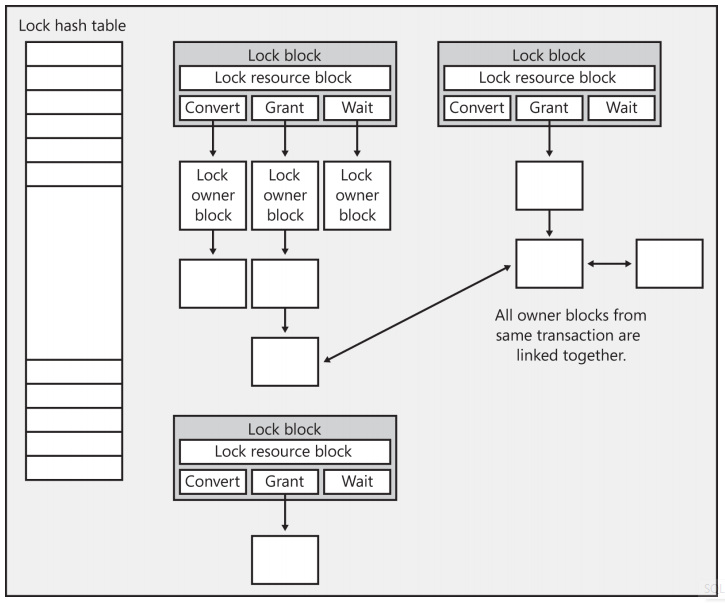
\includegraphics[width=0.85\textwidth]{image/fig_lock_manager_architecture.png}
    %\fbox{\parbox[c][3.8cm][c]{0.88\textwidth}{\centering \small \textbf{[Figure 2.1 Placeholder: SQL Server Lock Manager In-Memory Structure]}\\[1.5mm] \footnotesize Recommended Source: Microsoft Learn -- \textsl{SQL Server Transaction Locking and Row Versioning Guide} / Kalen Delaney, \textsl{SQL Server Internals}. Diagram showing Lock Hash Table Buckets pointing to Lock Resource Heads ($\approx$96B) and granted/waiting Lock Owner chains ($\approx$64B).}}
    \caption{Internal Architecture of the Microsoft SQL Server In-Memory Lock Manager}
    \label{fig:lock_manager_arch}
\end{figure}

\subsection{Lock Resource Granularity Hierarchy}
To balance concurrency throughput against lock memory overhead across both point lookups and massive table scans, SQL Server establishes a five-tier lock resource hierarchy:
\begin{equation}
    \text{DATABASE} \longrightarrow \text{OBJECT (Table/View)} \longrightarrow \text{HOBT / EXTENT} \longrightarrow \text{PAGE} \longrightarrow \text{KEY / RID}
\end{equation}
\begin{itemize}
    \item \textbf{DATABASE:} Prevents database dropping or schema alterations during active user sessions.
    \item \textbf{OBJECT:} Protects complete relational tables, indexed views, or system catalogs.
    \item \textbf{HOBT (Heap or B-Tree) / EXTENT:} Locks allocation units or physical 64KB extents (8 contiguous 8KB pages).
    \item \textbf{PAGE:} Locks individual 8KB leaf or intermediate B-Tree index pages.
    \item \textbf{KEY:} Fine-grained lock targeting a 6-byte hash representing an indexed key in a clustered or non-clustered B-Tree index.
    \item \textbf{RID (Row Identifier):} Fine-grained lock addressing a single record on an unindexed heap table using a \code{FileID:PageID:SlotNumber} tuple.
\end{itemize}

\begin{figure}[H]
    \centering
    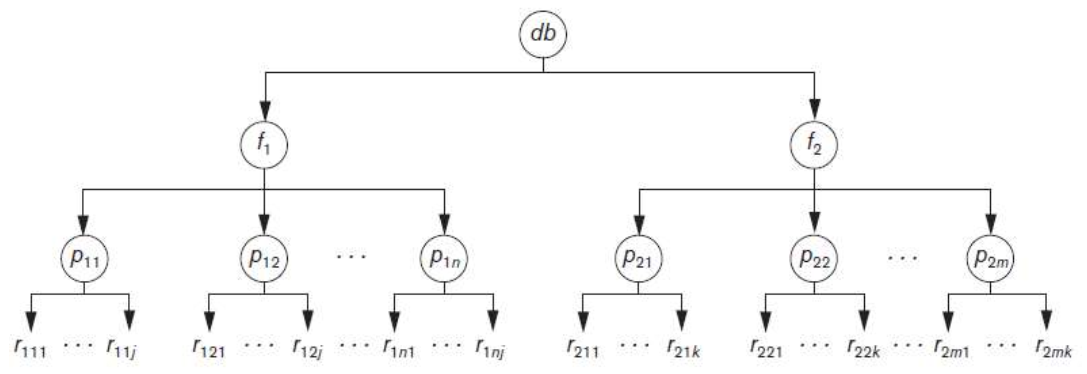
\includegraphics[width=0.75\textwidth]{image/fig_granularity_hierarchy.png}
    %\fbox{\parbox[c][3.8cm][c]{0.88\textwidth}{\centering \small \textbf{[Figure 2.2 Placeholder: Multiple Granularity Locking (MGL) Hierarchy Tree]}\\[1.5mm] \footnotesize Recommended Source: Elmasri et al., \textsl{Fundamentals of Database Systems}, Chapter 5, Slide 52 / Figure 21.8. Tree diagram showing granularity traversal from Database ($db$) down through Table/File ($f$), Pages ($p$), and Records/Keys ($r$).}}
    \caption{Multiple Granularity Tree Hierarchy in Database Locking (adapted from Elmasri et al.)}
    \label{fig:mgl_hierarchy}
\end{figure}

\subsection{Operational Lock Modes and Compatibility}
SQL Server provides specialized lock modes tailored to specific relational operations:
\begin{itemize}
    \item \textbf{Shared Lock ($S$):} Acquired by read operations (\code{SELECT}). Multiple concurrent transactions can hold concurrent $S$-locks on the same resource. Under \code{READ COMMITTED}, $S$-locks are dropped as soon as the cursor advances; under \code{REPEATABLE READ} or \code{SERIALIZABLE}, they are retained until commit.
    \item \textbf{Exclusive Lock ($X$):} Acquired by data-modification statements (\code{INSERT}, \code{UPDATE}, \code{DELETE}). $X$-locks are strictly incompatible with all other modes, preventing concurrent reads or writes until transaction commit or rollback.
    \item \textbf{Update Lock ($U$):} A hybrid asymmetric lock engineered to eliminate conversion deadlocks. When evaluating an \code{UPDATE} statement with a search predicate, the engine initially places $U$-locks on candidate rows during scanning. Multiple transactions cannot hold concurrent $U$-locks on the same row, but readers holding $S$-locks are permitted. Upon identifying qualifying target rows, the engine atomically converts the $U$-lock to an $X$-lock.
\end{itemize}

\subsection{Hierarchical Intention Locks (IS, IX, SIX, UIX)}
If locks were applied solely at the row level, a transaction executing an administrative table lock would be forced to inspect hundreds of thousands of row descriptors across all data pages. SQL Server eliminates this traversal overhead through \textbf{Intention Locks}:
\begin{itemize}
    \item \textbf{Intention Shared (IS):} Signals that fine-grained $S$-locks are held on descendant child items (rows or pages).
    \item \textbf{Intention Exclusive (IX):} Signals an intention to modify descendant child items via fine-grained $X$-locks.
    \item \textbf{Shared with Intention Exclusive (SIX):} Indicates the transaction holds a shared lock over the entire table while executing selective modifications on specific child rows via fine-grained $X$-locks.
    \item \textbf{Update with Intention Exclusive (UIX):} Applied at higher levels during update scans on descendant records.
\end{itemize}

\begin{table}[H]
\centering
\small
\caption{Hierarchical Lock Compatibility Matrix in Microsoft SQL Server}
\label{tab:mssql_lock_compatibility}
\begin{tabularx}{\textwidth}{@{}lcccccc@{}}
\toprule
\textbf{Held Mode $\backslash$ Requested Mode} & \textbf{IS} & \textbf{IX} & \textbf{S} & \textbf{SIX} & \textbf{U} & \textbf{X} \\ \midrule
\textbf{Intention Shared (IS)} & Granted & Granted & Granted & Granted & Granted & Blocked \\
\textbf{Intention Exclusive (IX)} & Granted & Granted & Blocked & Blocked & Blocked & Blocked \\
\textbf{Shared (S)} & Granted & Blocked & Granted & Blocked & Granted & Blocked \\
\textbf{Shared-Intention-Exclusive (SIX)} & Granted & Blocked & Blocked & Blocked & Blocked & Blocked \\
\textbf{Update (U)} & Granted & Blocked & Granted & Blocked & Blocked & Blocked \\
\textbf{Exclusive (X)} & Blocked & Blocked & Blocked & Blocked & Blocked & Blocked \\ \bottomrule
\end{tabularx}
\end{table}

\subsection{Key-Range Locking Architecture on B-Tree Indexes}
Under the \code{SERIALIZABLE} isolation level, evaluating predicate logic by evaluating arbitrary boolean formulas in memory (predicate locking) imposes severe CPU overhead. SQL Server maps logical intervals directly onto physical B-Tree index structures via \textbf{Key-Range Locks}:
\begin{itemize}
    \item \textbf{\code{RangeS-S}:} Shared lock on the key range interval and a shared lock on the bounding key, protecting range reads.
    \item \textbf{\code{RangeS-U}:} Shared range lock with an Update ($U$) lock on the bounding key, used during update candidate scans.
    \item \textbf{\code{RangeI-N}:} Insert range lock with a null bounding key, applied during \code{INSERT} statements to verify that the new key does not collide with an active serializable range.
    \item \textbf{\code{RangeX-X}:} Exclusive range lock with an exclusive bounding key, used when updating or deleting keys inside a protected range.
\end{itemize}

\subsection{Schema Locks (Sch-S and Sch-M)}
\begin{itemize}
    \item \textbf{Schema Stability Lock (Sch-S):} Acquired by the query processor during compilation and execution. It blocks DDL statements (\code{ALTER TABLE}, \code{DROP TABLE}) from modifying table schema while queries run, but is compatible with all operational data locks ($S$, $X$).
    \item \textbf{Schema Modification Lock (Sch-M):} Acquired during structural DDL operations and index rebuilds. Sch-M is strictly incompatible with all other lock modes, completely blocking concurrent queries until the structural alteration completes.
\end{itemize}

\subsection{Engine Lock Escalation Algorithm and Heuristics}
Maintaining fine-grained locks across massive tables consumes substantial non-swappable physical RAM within the buffer pool ($\approx$96 bytes per resource and $\approx$64 bytes per owner). To prevent out-of-memory states, SQL Server triggers \textbf{Lock Escalation}:
\begin{itemize}
    \item \textbf{Trigger Thresholds:} Escalation evaluates when a single query accumulates more than \textbf{5,000 discrete locks} on a single table partition, or when lock memory consumption exceeds 24\% to 40\% of the allocated buffer pool.
    \item \textbf{Trade-off Dynamics:} Converting thousands of fine-grained row/page locks into a single table lock (\code{OBJECT:\,S} or \code{OBJECT:\,X}) immediately reclaims memory and minimizes CPU hashing overhead, but severely curtails multi-user concurrency by serializing access to the entire table.
\end{itemize}



\subsection{Deadlock Detection and Engine Mitigation Mechanics}
\label{sec:r5-engine-deadlock-mvcc}

Table~\ref{tab:r5-methods} synthesizes the concrete mechanisms Microsoft SQL Server provides for deadlock resolution and multi-version concurrency control.

\begin{table}[H]
\centering
\caption{SQL Server mechanisms for deadlock handling and multi-version concurrency}
\label{tab:r5-methods}
\scriptsize
\setlength{\tabcolsep}{3pt}
\begin{tabularx}{\textwidth}{@{}c l >{\raggedright\arraybackslash}X >{\raggedright\arraybackslash}X@{}}
\toprule
\textbf{\#} & \textbf{Mechanism} & \textbf{Purpose} & \textbf{How it is used} \\
\midrule
M1  & Deadlock Monitor & Detect cycles in the waits-for graph automatically & Always on (background task) \\
M2  & Victim selection, \code{DEADLOCK\_PRIORITY} & Decide which transaction is rolled back & \code{SET DEADLOCK\_PRIORITY LOW | NORMAL | HIGH | -10..10} \\
M3  & Error 1205 + retry & Let the application recover from being the victim & \code{TRY\dots CATCH}, \code{ROLLBACK}, re-run \\
M4  & \code{LOCK\_TIMEOUT} & Bound the time a session waits for any lock & \code{SET LOCK\_TIMEOUT <ms>}, error 1222 \\
M5  & Deadlock diagnostics & Capture the deadlock graph for analysis & \code{system\_health} XE, \code{.xdl}, trace flag 1222 \\
M6  & Deadlock avoidance by design & Reduce the chance a cycle forms & access order, \code{UPDLOCK}, short transactions, indexes \\
M7  & Read Committed Snapshot (RCSI) & Readers never wait for writers at READ COMMITTED & \code{ALTER DATABASE \dots\ SET READ\_COMMITTED\_SNAPSHOT ON} \\
M8  & Snapshot Isolation (SI) & Transaction-wide consistent snapshot & \code{ALLOW\_SNAPSHOT\_ISOLATION ON} followed by \code{SET TRANSACTION ISOLATION LEVEL SNAPSHOT} \\
M9  & Version store & Storage and cleanup of row versions & \code{tempdb} (or PVS with ADR), automatic cleanup \\
M10 & \code{READCOMMITTEDLOCK} hint, DMVs & Opt out of RCSI per table; monitor versioning & table hint; \code{sys.dm\_tran\_version\_store\_space\_usage} \\
M11 & Optimized locking, In-Memory OLTP & Newer lock-light / lock-free engines & SQL Server 2025 + ADR; memory-optimized tables \\
\bottomrule
\end{tabularx}
\end{table}

\ReportBlock{M1 --- Deadlock Monitor (detection and resolution).}
\emph{Content and purpose:} SQL Server lets deadlocks happen and then breaks them, exactly the ``detection and resolution'' strategy of the slides. \emph{How the engine runs it:} a background thread, the \textbf{Lock Monitor}, searches the waits-for graph of all waiting tasks every 5~seconds by default. When it finds a deadlock, the search interval drops (down to 100~ms) and goes back to 5~s once deadlocks stop. Besides lock waits, the graph also includes waits on worker threads, memory and parallel-query resources. \emph{How to use it:} nothing to enable; the monitor is always running.

\ReportBlock{M2 --- Victim selection and \code{SET DEADLOCK\_PRIORITY}.}
\emph{Content:} the slides only say ``one transaction is selected as victim''. SQL Server applies two rules in order: (1) the session with the \textbf{lowest deadlock priority} is the victim; (2) at equal priority, the transaction that is \textbf{cheapest to roll back} (least transaction log used) is the victim; a remaining tie is broken arbitrarily. \emph{Purpose:} protect important work (e.g.\ a radiologist's sign-off) and keep the rollback cost small. \emph{How to use it:} \code{SET DEADLOCK\_PRIORITY LOW} ($-5$), \code{NORMAL} (0, default), \code{HIGH} (5) or any integer from $-10$ to $10$, per session. This also answers the slides' \emph{starvation} problem: a session that is always sacrificed can be given a higher priority.

\ReportBlock{M3 --- Error 1205 and retry.}
The victim's transaction is rolled back by the engine and its client receives \textbf{Msg 1205} (``\dots\ has been chosen as the deadlock victim. Rerun the transaction.''). The other transaction continues. Because the victim did nothing wrong, the standard pattern is \code{BEGIN TRY \dots\ COMMIT \dots\ END TRY BEGIN CATCH IF @@TRANCOUNT > 0 ROLLBACK; \dots\ END CATCH} plus an automatic retry when \code{ERROR\_NUMBER() = 1205}.

\ReportBlock{M4 --- \code{SET LOCK\_TIMEOUT}.}
\emph{Content and purpose:} by default a session waits for a lock forever (\code{-1}). \code{SET LOCK\_TIMEOUT n} makes any lock request give up after $n$~ms with \textbf{error 1222}. It does not detect deadlocks, but it limits how long a user waits and breaks long blocking chains (a timeout-based form of prevention, as mentioned in the slides). \emph{Important behaviour:} error 1222 cancels only the \emph{statement}; it does \emph{not} roll back the transaction, and rows already sent stay sent (observed in Section~\ref{sec:r5-2-queries}). The application must decide to roll back or retry.

\ReportBlock{M5 --- Deadlock diagnostics.}
Every deadlock is written as an \code{xml\_deadlock\_report} event by the built-in Extended Events session \textbf{\code{system\_health}} (always running). The XML lists the victim, every process with its \code{priority}, \code{logused}, wait resource and SQL text, and every resource with its owner and waiter. Saved as \code{.xdl}, it opens in SSMS as the graphical \textbf{Deadlock Graph}. Other options are trace flag 1222 (writes the same information to the error log), a custom Extended Events session, or the Deadlock graph event of SQL Profiler. Script: \code{01\_deadlock\_graph.sql}.

\ReportBlock{M6 --- Avoiding deadlocks by design.}
SQL Server does not implement wait-die or wound-wait, so avoidance is left to the developer: (a) access tables and rows in the \textbf{same order} in every transaction (e.g.\ always \code{Patients} then \code{MRI\_Scans}); (b) take the \textbf{update lock U} early with the \code{UPDLOCK} hint when a row is read and then updated, which prevents the S$\rightarrow$X \emph{conversion deadlock}, because U is not compatible with U; (c) keep transactions short with no user interaction inside; (d) create indexes so that statements lock only the rows they need (the lock footprint follows the execution plan, Section~\ref{sec:r5-2-queries}); (e) use RCSI so that readers no longer take part in deadlocks.

\ReportBlock{M7 --- Read Committed Snapshot Isolation (RCSI).}
\emph{Content:} a database option that changes how READ COMMITTED is implemented, with no change to the application code. \emph{How the engine runs it:} every UPDATE/DELETE copies the previous committed version of the row into the \textbf{version store} and links it from the row through a 14-byte versioning tag (transaction sequence number + pointer). A READ COMMITTED statement then takes \textbf{no S locks}: for each row it walks the version chain back to the version committed \emph{when the statement started}. Writers still take X locks between themselves (W--W conflicts are still serialised by locking). \emph{Purpose:} reads never block writes and writes never block reads, and there is still no dirty read. \emph{How to use it:} \code{ALTER DATABASE SpineMRI\_DBMS SET READ\_COMMITTED\_SNAPSHOT ON WITH ROLLBACK IMMEDIATE} (needs exclusive access). This is very close to the slides' \emph{multiversion 2PL}: readers read the committed version while a writer holds its lock, but without certify locks at commit time.

\ReportBlock{M8 --- Snapshot Isolation (SI).}
\emph{Content:} a separate isolation level. The snapshot is taken at the \textbf{first data access of the transaction}, so all reads of the transaction see the same committed state (transaction-level, whereas RCSI is statement-level). \emph{Concurrency rule:} if a SNAPSHOT transaction tries to modify a row that another transaction changed and committed after the snapshot started, the engine aborts it with \textbf{error 3960} (``first committer wins''). This plays the role of rule~1 of the slides' multiversion timestamp ordering: a write based on an outdated version is rejected, so no lost update is possible. \emph{How to use it:} \code{ALTER DATABASE \dots\ SET ALLOW\_SNAPSHOT\_ISOLATION ON}, then \code{SET TRANSACTION ISOLATION LEVEL SNAPSHOT} per session.

\ReportBlock{M9 --- Version store and its cleanup.}
Row versions live in \textbf{\code{tempdb}}; when Accelerated Database Recovery (ADR) is enabled they live in a \emph{Persistent Version Store} inside the user database instead. A background cleanup task removes versions that no active transaction can still need. This is the ``garbage collection'' of the slides, and also its side effect: extra storage and I/O, plus a long-running snapshot transaction can keep many versions alive.

\ReportBlock{M10 --- Fine control and monitoring.}
With RCSI on, the table hint \code{WITH (READCOMMITTEDLOCK)} makes one statement go back to locking reads (useful when a statement must see the very latest committed value). Version activity is visible in \code{sys.dm\_tran\_version\_store\_space\_usage} and \code{sys.dm\_tran\_active\_snapshot\_database\_transactions}.

\ReportBlock{M11 --- Other engines (not used in our database).}
SQL Server 2025 offers \emph{optimized locking} (transaction-ID locking and lock-after-qualification, built on ADR), which holds far fewer row locks for writers and therefore reduces blocking and deadlocks. Memory-optimized (In-Memory OLTP) tables use a lock-free, fully optimistic multi-version engine. Both are \textbf{off} in \code{SpineMRI\_DBMS} (\code{is\_optimized\_locking\_on = 0}, ADR off), so all results below show the classic behaviour.

\begin{table}[H]
\centering
\caption{Chapter 5 slides versus SQL Server}
\label{tab:r5-slides-vs-mssql}
\scriptsize
\begin{tabularx}{\textwidth}{l X X}
\toprule
\textbf{Topic} & \textbf{Slides} & \textbf{SQL Server} \\
\midrule
Deadlock strategy & Prevention, detection, avoidance (wait-die, wound-wait) & Detection and resolution only (Lock Monitor); avoidance left to design (M6) \\
Victim choice & ``a transaction of the cycle'' & Lowest \code{DEADLOCK\_PRIORITY}, then least log used \\
Starvation & Possible; wait-die/wound-wait avoid it & Controlled by \code{DEADLOCK\_PRIORITY} and application retry \\
Waiting limit & --- & \code{LOCK\_TIMEOUT}, error 1222 \\
Multiversion scheme & MV timestamp ordering; MV2PL with certify locks & RCSI (statement snapshot) and SI (transaction snapshot); writers keep X locks, no certify lock \\
Write conflict on versions & Abort $T$ if $read\_TS(X_i) > TS(T)$ & SI: abort with error 3960 (first committer wins) \\
Old versions & Garbage collection & Version store in \code{tempdb} / PVS, background cleanup \\
\bottomrule
\end{tabularx}
\end{table}

% =====================================================================

\section{Pessimistic Concurrency Analysis on Canonical Queries Q1--Q3}
\label{sec:r5-1-queries}
To evaluate engine-level locking behavior on real clinical data, we analyze the 3 Canonical Queries across the \code{SpineMRI\_DBMS} database (575 patients, 48,345 scans, and 48,345 feature vectors) using Dynamic Management Views (\code{sys.dm\_tran\_locks} and \code{sys.dm\_os\_waiting\_tasks}).

\subsection{Canonical Query 1: Single-Patient Point Lookup and Scan Retrieval}
\ReportBlock{Canonical Query Definition}
Retrieves clinical notes and associated MRI scan file paths for target patient \code{'0001'}:
\begin{SQLCode}
SELECT p.PatientID, p.PatientName, p.ClinicalNotes,
       s.ScanID, s.SeriesDescription, s.ImagePath
FROM Patients p
INNER JOIN MRI_Scans s ON p.PatientID = s.PatientID
WHERE p.PatientID = '0001';
\end{SQLCode}

\ReportBlock{Engine Locking and Plan Mechanics}
\begin{itemize}
    \item \textbf{Index Path and Cost Evaluation:} Because \code{PatientID} is the clustered primary key on \code{Patients} (\code{PK\_Patients}), the Query Optimizer selects a point \textbf{Clustered Index Seek} (estimated cardinality = 1). On \code{MRI\_Scans}, the foreign key index on \code{PatientID} permits a secondary index seek, joined via Nested Loops.
    \item \textbf{Lock Granularity Selected:} The Lock Manager acquires an \code{OBJECT:\,IS} lock on \code{Patients}, followed by a fine-grained \textbf{\code{KEY:\,S}} lock on the single clustered leaf entry for \code{PatientID = '0001'}. On \code{MRI\_Scans}, matching scan rows are protected with \code{KEY:\,S} locks under an \code{OBJECT:\,IS} container.
    \item \textbf{Isolation Level Mechanics:}
    \begin{itemize}
        \item Under default \code{READ COMMITTED}: The \code{KEY:\,S} lock is acquired to fetch data pages into the buffer pool and is \textbf{released immediately} upon operator completion, maximizing throughput for concurrent transactions.
        \item Under \code{REPEATABLE READ} / \code{SERIALIZABLE}: The \code{KEY:\,S} lock is retained for the entire duration of the transaction. Any concurrent session attempting to modify patient \code{'0001'} (\code{UPDATE Patients ... WHERE PatientID = '0001'}) requests an incompatible \code{KEY:\,X} lock and is placed into a \code{SUSPENDED} state in the FIFO queue until commit.
    \end{itemize}
\end{itemize}

\begin{figure}[H]
    \centering
    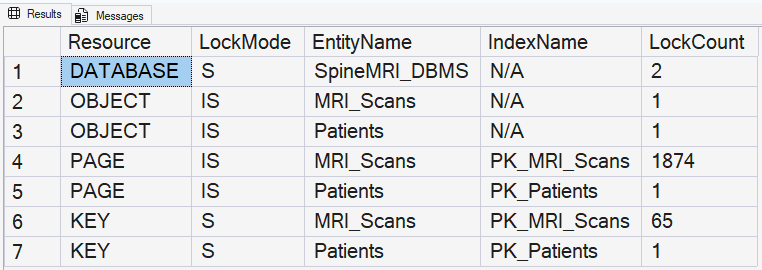
\includegraphics[width=0.88\textwidth]{image/fig_q1_dmv_locks.png}
    %\fbox{\parbox[c][3.8cm][c]{0.88\textwidth}{\centering \small \textbf{[Figure 2.3 Placeholder: SSMS Diagnostic Lock Table for Query 1]}\\[1.5mm] \footnotesize Recommended Source: SSMS query execution screenshot of \code{sys.dm\_tran\_locks} from Case 1 Option A in \code{05\_concurrency\_control\_role5.sql}. Displays the lock hierarchy summary: \code{DATABASE} (\code{S}), \code{OBJECT} (\code{IS} on \code{Patients} and \code{MRI\_Scans}), and \code{KEY} (\code{S} on \code{PK\_Patients} and \code{PK\_MRI\_Scans}) during an open transaction.}}
    \caption{Dynamic Management View (\code{sys.dm\_tran\_locks}) Lock Verification for Query 1 under \code{REPEATABLE READ}}
    \label{fig:q1_dmv_locks}
\end{figure}

\subsection{Canonical Query 2: Filtered Scan Retrieval by Pulse Sequence (T2 Sagittal)}
\ReportBlock{Canonical Query Definition}
Retrieves diagnostic narrative and scan paths restricted to T2 sagittal sequences (\code{\%T2\%SAG\%}) for a designated patient:
\begin{SQLCode}
SELECT p.PatientID, p.PatientName, p.ClinicalNotes,
       s.ScanID, s.SeriesDescription, s.ImagePath
FROM Patients p
INNER JOIN MRI_Scans s ON p.PatientID = s.PatientID
WHERE p.PatientID = '0001'
  AND s.SeriesDescription LIKE '%T2%SAG%';
\end{SQLCode}

\ReportBlock{Engine Locking and Phantom Read Dynamics}
\begin{itemize}
    \item \textbf{Predicate Processing and Filter Locks:} The engine performs an exact Clustered Index Seek on \code{Patients} for \code{'0001'}, followed by a join to \code{MRI\_Scans}. Because the string predicate contains a leading wildcard (\code{\%T2\%SAG\%}), the engine evaluates the non-key attribute filter on candidate rows matching \code{PatientID = '0001'}.
    \item \textbf{Phantom Read Vulnerability under REPEATABLE READ:} When executed inside a \code{REPEATABLE READ} transaction, SQL Server places \code{KEY:\,S} locks on all existing scan records for patient \code{'0001'}. However, if concurrent Session 2 inserts a \textit{new} T2 sagittal slice for patient \code{'0001'} and commits, Session 1's subsequent re-execution observes the newly inserted slice, suffering a \textbf{Phantom Read}.
    \item \textbf{Phantom Prevention under SERIALIZABLE:} Under \code{SERIALIZABLE}, the Lock Manager applies \textbf{\code{RangeS-S}} key-range locks covering the index key interval for \code{PatientID = '0001'} on the B-Tree leaf. If Session 2 attempts to insert a new scan row for patient \code{'0001'}, the engine requests a \code{RangeI-N} lock that conflicts with \code{RangeS-S}. Session 2 is blocked immediately until Session 1 finishes, eliminating phantom reads.
\end{itemize}

\begin{figure}[H]
    \centering
    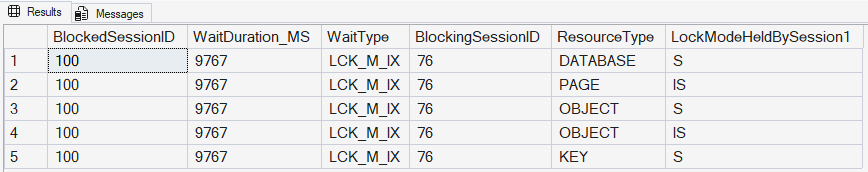
\includegraphics[width=0.88\textwidth]{image/fig_q2_phantom_lock.png}
    %\fbox{\parbox[c][3.8cm][c]{0.88\textwidth}{\centering \small \textbf{[Figure 2.4 Placeholder: SSMS Key-Range Lock \& Blocked Session Monitor for Query 2]}\\[1.5mm] \footnotesize Recommended Source: SSMS query screenshot of \code{sys.dm\_tran\_locks} and \code{sys.dm\_os\_waiting\_tasks} from Case 2 in \code{05\_concurrency\_control\_role5.sql}. Displays Session 1 holding \code{RangeS-S} locks on B-Tree keys while Session 2 is blocked with wait type \code{LCK\_M\_RANGEI\_N} on \code{MRI\_Scans}.}}
    \caption{Key-Range Locking (\code{RangeS-S}) and Phantom Insertion Blocking under \code{SERIALIZABLE} in Query 2}
    \label{fig:q2_phantom_lock}
\end{figure}

\subsection{Canonical Query 3: AI Feature Similarity Retrieval (Content-Based Search)}
\ReportBlock{Canonical Query Definition}
Calculates mathematical Euclidean distance across normalized AI feature embeddings (\code{V\_Dim1..V\_Dim4}) over all 48,345 slices to retrieve top-3 visually similar scans:
\begin{SQLCode}
DECLARE @TargetScanID INT = 1;
DECLARE @T1 FLOAT, @T2 FLOAT, @T3 FLOAT, @T4 FLOAT;

SELECT @T1 = V_Dim1, @T2 = V_Dim2, @T3 = V_Dim3, @T4 = V_Dim4 
FROM Image_Features WHERE ScanID = @TargetScanID;

SELECT TOP 3 s.ScanID, s.PatientID, s.SeriesDescription, s.ImagePath,
    SQRT(SQUARE(f.V_Dim1 - @T1) + SQUARE(f.V_Dim2 - @T2) + 
         SQUARE(f.V_Dim3 - @T3) + SQUARE(f.V_Dim4 - @T4)) AS EuclideanDistance
FROM Image_Features f
INNER JOIN MRI_Scans s ON f.ScanID = s.ScanID
WHERE f.ScanID <> @TargetScanID
ORDER BY EuclideanDistance ASC;
\end{SQLCode}

\ReportBlock{Engine Locking and Lock Escalation Dynamics}
\begin{itemize}
    \item \textbf{Full Table Scan Requirements:} Because calculating non-linear Euclidean distance ($\sqrt{\sum (u_k - v_k)^2}$) requires computing arithmetic differences across every row, standard B-Tree indexes cannot filter the calculation via seeks. The Query Optimizer executes a \textbf{Clustered Index Scan} over all 48,345 rows in \code{Image\_Features}, followed by a \code{Top N Sort}.
    \item \textbf{Lock Granularity Traversal:} During the scan phase under default \code{READ COMMITTED}, SQL Server places an \code{OBJECT:\,IS} lock on \code{Image\_Features} and traverses 8KB pages, acquiring and releasing \code{PAGE:\,S} locks in rapid succession. Because locks are dropped as pages are processed, memory consumption remains negligible.
    \item \textbf{Lock Escalation Exposure on the Ingested Clinical Database:} On the full production database of 48,345 scans, if this query is executed within an open transaction under \code{REPEATABLE READ} or \code{SERIALIZABLE}, the engine must retain shared locks on every accessed page. When the number of accumulated locks crosses the 5,000 threshold, the Lock Manager triggers \textbf{Lock Escalation}, converting thousands of fine-grained page/key locks into a single \textbf{\code{OBJECT:\,S}} table lock. This reclaims memory in the buffer pool, but blocks all concurrent transactional modifications (\code{INSERT}, \code{UPDATE}) on the entire \code{Image\_Features} table.
\end{itemize}

\begin{figure}[H]
    \centering
    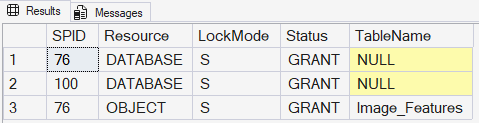
\includegraphics[width=0.88\textwidth]{image/fig_q3_execution_escalation.png}
    %\fbox{\parbox[c][3.8cm][c]{0.88\textwidth}{\centering \small \textbf{[Figure 2.5 Placeholder: SSMS Execution Plan and Lock Escalation Event for Query 3]}\\[1.5mm] \footnotesize Recommended Source: SSMS graphical execution plan showing the 48,345-row Clustered Index Scan on \code{Image\_Features} with Top-N Sort, combined with a \code{sys.dm\_tran\_locks} screenshot showing escalated \code{OBJECT:\,S} lock from Case 3 in \code{05\_concurrency\_control\_role5.sql}.}}
    \caption{Execution Plan Operators and Lock Escalation Footprint for Query 3 Vector Distance Search}
    \label{fig:q3_escalation}
\end{figure}

\section{Synthesis: ANSI SQL Isolation Levels vs. MSSQL Engine Mechanics}
Table~\ref{tab:ansi_mssql_matrix} synthesizes theoretical isolation levels, potential data anomalies, and Microsoft SQL Server's concrete engine-level locking behavior across the clinical imaging workload.

\begin{table}[H]
\centering
\small
\caption{ANSI SQL Isolation Levels and Concrete MSSQL Engine Locking Behaviors}
\label{tab:ansi_mssql_matrix}
\begin{tabularx}{\textwidth}{@{}l ccc >{\raggedright\arraybackslash}X@{}}
\toprule
\textbf{Isolation Level} & \textbf{\shortstack{Dirty\\Read}} & \textbf{\shortstack{Non-repeatable\\Read}} & \textbf{\shortstack{Phantom\\Read}} & \textbf{Concrete MSSQL Engine Locking Behavior} \\ \midrule
\textbf{READ UNCOMMITTED} & Yes & Yes & Yes & Executes reads without acquiring $S$-locks; ignores active $X$-locks held by concurrent writers. \\ \addlinespace[4pt]
\textbf{READ COMMITTED}   & No  & Yes & Yes & Acquires fine-grained $S$-locks, but releases them immediately after statement execution. \\ \addlinespace[4pt]
\textbf{REPEATABLE READ}  & No  & No  & Yes & Retains fine-grained $S$-locks on accessed keys/pages until transaction termination. \\ \addlinespace[4pt]
\textbf{SERIALIZABLE}     & No  & No  & No  & Applies \textbf{Key-Range Locks} (\code{RangeS-S}) on B-Tree intervals to prevent phantom insertions. \\ \bottomrule
\end{tabularx}
\end{table}

\section{Empirical Deadlock Resolution and MVCC Evaluation}
\label{sec:r5-2-experiments}

\subsection{Experimental Environment and Diagnostic Harness}
\label{sec:r5-2-setup}

\begin{itemize}
  \item \textbf{Engine:} Microsoft SQL Server 2025 (RTM) 17.0.1000.7 Developer Edition, compatibility level 170; database restored from \code{data/SpineMRI\_DBMS.bak} (575 patients, 48{,}345 scans). ADR, optimized locking, RCSI and SNAPSHOT are OFF at the start.
  \item \textbf{Two sessions:} each scenario has a Session A file and a Session B file in \code{scripts/sql/role5/}, opened in two SSMS windows. The session that holds locks contains a \code{WAITFOR DELAY} so the presenter can switch window. A third window may run \code{03\_lock\_monitor.sql}, which shows the waits-for edges (\code{sys.dm\_exec\_requests.blocking\_session\_id}) and the lock table (\code{sys.dm\_tran\_locks}).
  \item \textbf{Measurements:} \emph{elapsed time} of the statement, and \emph{lock wait time} taken from \code{sys.dm\_exec\_session\_wait\_stats} (sum of \code{LCK\_M\_*} waits of the session, before/after the statement). The number of locks a query requests per table comes from \code{sys.dm\_db\_index\_operational\_stats} (\code{row\_lock\_count}, \code{page\_lock\_count}). For the reported numbers the same files were launched as parallel \code{sqlcmd} sessions (B started 2~s after A); raw logs are in \code{scripts/sql/role5/evidence/run\_logs/}. \code{99\_reset.sql} restores the data after each run.
\end{itemize}

% =====================================================================
\subsection{Experiment 1: Deadlock Induction, Victim Selection, and Deadlock Graph Analysis}
\label{sec:r5-2-deadlock}

\textbf{Scenario.} Two staff members update the data that Query~1 returns, in opposite order. Session A (radiologist) updates patient \code{0001}, then the slice \code{ScanID = 1} of that patient; Session B (technician) updates slice \code{1}, then patient \code{0001}. Both use \code{TRY\dots CATCH} with \code{ROLLBACK}.

\begin{SQLCode}
-- Session A (01_deadlock_A.sql)                -- Session B (01_deadlock_B.sql)
SET DEADLOCK_PRIORITY NORMAL;  -- run 2: LOW    SET DEADLOCK_PRIORITY NORMAL;
BEGIN TRANSACTION;                              BEGIN TRANSACTION;
UPDATE dbo.Patients SET DiagnosisStatus =       UPDATE dbo.MRI_Scans
  'Under Review' WHERE PatientID = '0001';        SET AcquisitionDate = SYSDATETIME()
WAITFOR DELAY '00:00:06';                         WHERE ScanID = 1;
UPDATE dbo.MRI_Scans                            WAITFOR DELAY '00:00:02';
  SET AcquisitionDate = SYSDATETIME()           UPDATE dbo.Patients SET DiagnosisStatus =
  WHERE ScanID = 1;          -- waits for B       'Image Checked' WHERE PatientID = '0001';
COMMIT TRANSACTION;                             COMMIT TRANSACTION;  -- waits for A
\end{SQLCode}

The lock monitor captured the cycle of the waits-for graph before the Lock Monitor broke it (run 1, session 62 = A, 63 = B):

\begin{SQLCode}
WaitingSession BlockedBy wait_type WaitMs WaitingStatement
62             63        LCK_M_X   270    UPDATE [dbo].[MRI_Scans] ... WHERE [ScanID]=@1
63             62        LCK_M_X   2236   UPDATE [dbo].[Patients]  ... WHERE [PatientID]=@2

SessionID Resource ObjectName IndexName     KeyHash         Mode Status
62        KEY      Patients   PK_Patients   (5f6f76815dbe)  X    GRANT
62        KEY      MRI_Scans  PK_MRI_Scans  (8194443284a0)  X    WAIT
63        KEY      MRI_Scans  PK_MRI_Scans  (8194443284a0)  X    GRANT
63        KEY      Patients   PK_Patients   (5f6f76815dbe)  X    WAIT
\end{SQLCode}

The edges $62 \rightarrow 63$ and $63 \rightarrow 62$ form exactly the cycle of the slides' wait-for graph. Table~\ref{tab:r5-deadlock} gives the outcome of two runs, using the values read from the captured \code{xml\_deadlock\_report} events.

\begin{table}[H]
\centering
\caption{Experiment 1: victim selection (values from the deadlock graph XML)}
\label{tab:r5-deadlock}
\small
\begin{tabular}{lcccccc}
\toprule
\multirow{2}{*}{\textbf{Run}} & \multicolumn{2}{c}{\textbf{Session A}} & \multicolumn{2}{c}{\textbf{Session B}} & \multirow{2}{*}{\textbf{Victim}} & \textbf{Cycle $\rightarrow$} \\
 & priority & log used (bytes) & priority & log used (bytes) & & \textbf{resolved} \\
\midrule
1: NORMAL / NORMAL & 0  & 308 & 0 & 272 & B (error 1205) & 1.83 s \\
2: LOW / NORMAL    & $-5$ & 308 & 0 & 272 & A (error 1205) & 1.21 s \\
\bottomrule
\end{tabular}
\end{table}

\textbf{Analysis.} In run~1 both priorities are equal, so SQL Server applies the second rule and sacrifices B, which has written less log (272 vs.\ 308 bytes) and is cheaper to roll back. In run~2 A has a lower priority, and A becomes the victim \emph{even though it is the more expensive one to roll back}: priority is checked before cost. In both runs the victim received Msg 1205, its update was undone, and the survivor's blocked statement was granted and committed. The cycle was broken 1.2--1.8~s after it formed, which fits the 5-second search interval of the Lock Monitor. Figure~\ref{fig:r5-deadlock-tikz} redraws the graph of run~1 from \code{evidence/deadlock\_run1\_priority\_normal.xdl}; Figures~\ref{fig:r5-deadlock-ssms} and~\ref{fig:r5-deadlock-ssms-run2} are the graphs of run~1 and run~2 rendered by SSMS.

\begin{figure}[H]
\centering
\begin{tikzpicture}[
  proc/.style={ellipse, draw, thick, minimum width=36mm, minimum height=13mm, align=center, font=\small},
  res/.style={rectangle, draw, thick, fill=black!4, minimum width=40mm, minimum height=13mm, align=center, font=\small},
  lab/.style={font=\scriptsize, fill=white, inner sep=1pt},
  >=Stealth]
  \node[proc] (A) at (0,0) {Process 62 (Session A)\\ survivor, \code{logused} 308};
  \node[proc] (B) at (9,0) {Process 63 (Session B)\\ \textbf{victim}, \code{logused} 272};
  \node[res]  (P) at (4.5,2.2)  {Key lock \code{PK\_Patients}\\ \code{Patients} (0001)};
  \node[res]  (S) at (4.5,-2.2) {Key lock \code{PK\_MRI\_Scans}\\ \code{MRI\_Scans} (ScanID 1)};
  \draw[->, thick] (P) -- node[lab, above left]  {Owner mode: X} (A);
  \draw[->, thick, dashed] (B) -- node[lab, above right] {Request mode: X} (P);
  \draw[->, thick] (S) -- node[lab, below right] {Owner mode: X} (B);
  \draw[->, thick, dashed] (A) -- node[lab, below left] {Request mode: X} (S);
  \draw[red!70!black, very thick] ($(B)+(-1.9,-0.75)$) -- ($(B)+(1.9,0.75)$);
  \draw[red!70!black, very thick] ($(B)+(-1.9,0.75)$) -- ($(B)+(1.9,-0.75)$);
\end{tikzpicture}
\caption{Deadlock graph of run 1, redrawn from the \code{xml\_deadlock\_report} of \code{system\_health}. Solid arrows: lock owned; dashed arrows: lock requested. The two requests close the cycle; the crossed process is the victim.}
\label{fig:r5-deadlock-tikz}
\end{figure}

\begin{figure}[H]
  \centering
  \rolefivefig{image/role_5/role5_deadlock_graph_ssms.png}{\textwidth}{SSMS Deadlock Graph: open scripts/sql/role5/evidence/deadlock\_run1\_priority\_normal.xdl in SSMS}
  \caption{Deadlock Graph rendered by SSMS from \code{deadlock\_run1\_priority\_normal.xdl}. Ovals are processes (sessions), rectangles are the locked resources (key locks on \code{PK\_Patients} and \code{PK\_MRI\_Scans}). An arrow from a resource to a process means ``Owner Mode: X'' (the process holds it); an arrow from a process to a resource means ``Request Mode: X'' (the process waits for it). Process 63 (Session B, Log Used 272) is crossed out as the victim; process 62 (Session A, Log Used 308) survives; both have Deadlock priority 0.}
  \label{fig:r5-deadlock-ssms}
\end{figure}

\begin{figure}[H]
  \centering
  \rolefivefig{image/role_5/role5_deadlock_graph_ssms_run2_low.png}{\textwidth}{SSMS Deadlock Graph of run 2: open scripts/sql/role5/evidence/deadlock\_run2\_A\_priority\_low.xdl in SSMS}
  \caption{Deadlock Graph of run 2 (\code{deadlock\_run2\_A\_priority\_low.xdl}): the same cycle, but Session A now runs with \code{SET DEADLOCK\_PRIORITY LOW}. Process 62 (Session A, Deadlock priority $-5$, Log Used 308) is crossed out as the victim, although it is the \emph{more} expensive transaction to roll back; process 63 (Session B, priority 0, Log Used 272) survives. Priority is evaluated before rollback cost.}
  \label{fig:r5-deadlock-ssms-run2}
\end{figure}

% =====================================================================
\subsection{Experiment 2: Lock Wait Time Benchmarking --- Classic Locking versus RCSI}
\label{sec:r5-2-rcsi}

\textbf{Scenario.} Session A updates the diagnosis of patient \code{0001} and keeps the transaction open for 10~s (X lock held). Session B reads the same row at READ COMMITTED. The same pair of scripts is run three times with RCSI OFF and three times with RCSI ON (\code{02\_rcsi\_0\_enable\_row\_versioning.sql}).

\begin{SQLCode}
-- Session A (02_rcsi_A_writer.sql)
BEGIN TRANSACTION;
    UPDATE dbo.Patients SET DiagnosisStatus = 'Revised' WHERE PatientID = '0001';
    WAITFOR DELAY '00:00:10';
COMMIT TRANSACTION;

-- Session B (02_rcsi_B_reader.sql)
SET TRANSACTION ISOLATION LEVEL READ COMMITTED;
SELECT @v = DiagnosisStatus FROM dbo.Patients WHERE PatientID = '0001';
-- + elapsed time and LCK_M_* wait time from sys.dm_exec_session_wait_stats
\end{SQLCode}

\begin{table}[H]
\centering
\caption{Experiment 2: lock wait time of the reader, same scenario, 3 runs each}
\label{tab:r5-lockwait}
\small
\begin{tabular}{lccccl}
\toprule
\textbf{Mode} & \textbf{Run} & \textbf{Value read} & \textbf{Elapsed (ms)} & \textbf{Lock wait (ms)} & \textbf{Wait type} \\
\midrule
\multirow{3}{*}{Locking READ COMMITTED (RCSI OFF)} & 1 & \code{Revised} & 7{,}931 & 7{,}930 & \code{LCK\_M\_S} \\
 & 2 & \code{Revised} & 7{,}931 & 7{,}930 & \code{LCK\_M\_S} \\
 & 3 & \code{Revised} & 7{,}953 & 7{,}953 & \code{LCK\_M\_S} \\
\midrule
\multirow{3}{*}{READ COMMITTED SNAPSHOT (RCSI ON)} & 1 & \code{Confirmed} & 0 & 0 & --- \\
 & 2 & \code{Confirmed} & 0 & 0 & --- \\
 & 3 & \code{Confirmed} & 0 & 0 & --- \\
\midrule
\textbf{Average locking / RCSI} & & & \textbf{7{,}938 / 0} & \textbf{7{,}938 / 0} & \\
\bottomrule
\end{tabular}
\end{table}

\textbf{Analysis.} With classic locking, B's S request on key \code{(5f6f76815dbe)} is incompatible with A's X lock; the monitor shows \code{X GRANT} for A and \code{S WAIT} for B, and B waits until A commits (about 8~s, because B started 2~s after A), then reads the new value \code{Revised}. With RCSI the lock table during the same moment contains \emph{only} A's \code{IX/IX/X} locks --- B requests no S lock at all --- and \code{sys.dm\_tran\_version\_store\_space\_usage} reports \textbf{8 pages (64~KB)} of row versions. B immediately reads \code{Confirmed}, the last \emph{committed} version taken from the version store. Neither mode ever returns an uncommitted value. The trade-off: RCSI removes the waiting but may return a version that is a few seconds older.

\textbf{Snapshot Isolation (\code{02\_snapshot\_B\_reader.sql}).} A SNAPSHOT transaction read patient \code{0001} at the start (0~ms, \code{Confirmed}), waited while A committed \code{Revised}, and read again: the second read still returned \code{Confirmed}, while the committed value was already \code{Revised}. This shows the transaction-level snapshot of SI, versus the statement-level snapshot of RCSI.

\textbf{Update conflict (\code{02\_snapshot\_C\_update\_conflict.sql}).} A SNAPSHOT transaction read the row, A updated and committed it, and the snapshot transaction then tried to update it. SQL Server refused with \textbf{error 3960} (``Snapshot isolation transaction aborted due to update conflict \dots''). Under versioning, a write--write conflict is therefore resolved by aborting rather than by waiting, and no lost update can happen.

% =====================================================================
\subsection{Experiment 3: Canonical Queries Q1--Q3 under Active Concurrent Writers}
\label{sec:r5-2-queries}

This experiment applies the mechanisms above to the three canonical queries. Session A (\code{04\_queries\_A\_writer.sql}) re-labels one slice of \textbf{patient \code{0002}} (\code{ScanID = 80}) and keeps its X locks for 10~s before rolling back. Patient \code{0002} is \emph{not} in the result of Q1 or Q2 (which ask for patient \code{0001}) and is one of the 48{,}345 rows that Q3 compares. Session B runs Q1, Q2 or Q3 unchanged (\code{04\_queries\_B\_Q1/Q2/Q3.sql}). Every combination of two index states (\emph{PK only}, as in the backup; \emph{PK + covering}, with Role~2's index \code{IX\_MRIScans\_PatientID\_Covering (PatientID, SeriesDescription) INCLUDE (ImagePath)}) and two modes (locking, RCSI) was run, each query once alone (lock footprint) and once against the writer (blocking).

\begin{table}[H]
\centering
\caption{Access path chosen by the optimizer (estimated plans, \code{SHOWPLAN\_TEXT})}
\label{tab:r5-plans}
\scriptsize
\begin{tabularx}{\textwidth}{l X X}
\toprule
\textbf{Query} & \textbf{PK only} & \textbf{PK + covering index} \\
\midrule
Q1 & Nested Loops: Clustered Index \textbf{Seek} \code{PK\_Patients} + Clustered Index \textbf{Scan} \code{PK\_MRI\_Scans} (filter \code{PatientID='0001'}) & Nested Loops: Clustered Index Seek \code{PK\_Patients} + Index \textbf{Seek} \code{IX\_MRIScans\_PatientID\_Covering} \\
Q2 & Same as Q1, plus the \code{LIKE '\%T2\%SAG\%'} filter in the scan & Same as Q1; \code{LIKE} becomes a residual predicate of the seek \\
Q3 & Parallel Hash Match: Clustered Index \textbf{Scan} \code{PK\_Image\_Features} + Clustered Index \textbf{Scan} \code{PK\_MRI\_Scans}, then Top-N Sort & Same, but \code{MRI\_Scans} is read by an Index \textbf{Scan} of the narrower covering index \\
\bottomrule
\end{tabularx}
\end{table}

\begin{table}[H]
\centering
\caption{Concurrency behaviour of the canonical queries while a writer holds X locks on one row of patient 0002. Locks requested by the query alone at locking READ COMMITTED: r = row locks, p = page locks, (P) = \code{Patients}, (F) = \code{Image\_Features}. Under RCSI every query requested 0 locks. Times in ms.}
\label{tab:r5-queries}
\small
\setlength{\tabcolsep}{4pt}
\begin{tabular}{llllrrrr}
\toprule
\multirow{2}{*}{\textbf{Index}} & \multirow{2}{*}{\textbf{Q}} & \multicolumn{2}{c}{\textbf{Locks requested}} & \multicolumn{2}{c}{\textbf{Locking RC}} & \multicolumn{2}{c}{\textbf{RCSI}} \\
 & & \textbf{MRI\_Scans} & \textbf{Other table} & \textbf{Elapsed} & \textbf{Lock wait} & \textbf{Elapsed} & \textbf{Lock wait} \\
\midrule
\multirow{3}{*}{PK only}
 & Q1 & 1{,}874 p & 1 r + 1 p (P) & 7{,}976 & 7{,}969 & 5  & 0 \\
 & Q2 & 1{,}874 p & 1 r + 1 p (P) & 7{,}982 & 7{,}976 & 7  & 0 \\
 & Q3 & 1{,}903 p & 1 r + 3{,}780 p (F) & 7{,}983 & 7{,}972 & 16 & 0 \\
\midrule
\multirow{3}{*}{PK + covering}
 & Q1 & 65 r + 3 p & 1 r + 1 p (P) & 1 & 0 & 1  & 0 \\
 & Q2 & 65 r + 3 p & 1 r + 1 p (P) & 1 & 0 & 1  & 0 \\
 & Q3 & 1{,}588 p & 1 r + 3{,}780 p (F) & 7{,}993 & 7{,}982 & 17 & 0 \\
\bottomrule
\end{tabular}
\end{table}

\textbf{How SQL Server decides, query by query.}

\begin{itemize}
  \item \textbf{The optimizer chooses the plan by cost, and the plan decides the lock footprint.} The Query Optimizer does not consider concurrency; it picks the cheapest access path (Table~\ref{tab:r5-plans}). At run time the storage engine then chooses the \textbf{lock granularity from the access method}: for a \emph{scan} it requests \textbf{page locks} (one lock per 8~KB page instead of one per row, e.g.\ 1{,}874 page locks and 0 row locks on \code{MRI\_Scans}), for a \emph{seek} it requests \textbf{row (key) locks} plus intent locks on the few pages visited (65 key locks + 3 page locks). Under locking READ COMMITTED each S lock is released right after the row/page is read, so no lock escalation occurs even for Q3.

  \item \textbf{Q1 and Q2 with PK only: blocked by a patient they do not return.} Without an index on \code{MRI\_Scans.PatientID}, Q1 and Q2 must scan the whole table and test every row. When the scan reaches the page of \code{ScanID 80}, its page S lock conflicts with the writer's IX/X locks, so the query waits $\approx$8~s for a row of patient \code{0002}. With \code{LOCK\_TIMEOUT 3000} (\code{01\_lock\_timeout\_B\_Q1.sql}) the same Q1 had already streamed all 65 rows of patient \code{0001} (they are on the first pages) and then failed with error 1222 after 3{,}008~ms: SQL Server cannot know there are no more \code{0001} rows until the scan is finished.

  \item \textbf{Q1 and Q2 with the covering index: no blocking at all, even under locking.} The seek visits only the key range \code{PatientID = '0001'} of the index, so it never touches the locked row of patient \code{0002}. A good index therefore reduces blocking and deadlock risk as much as it reduces I/O. For Q2 the \code{LIKE '\%T2\%SAG\%'} test is a residual predicate: the 65 keys of the patient are still locked and read, then 15 rows are returned.

  \item \textbf{Q3: always blocked under locking.} Q3 must compare the reference vector with every other slice, so both tables are scanned completely (3{,}780 page locks on \code{Image\_Features}, 1{,}588--1{,}903 on \code{MRI\_Scans}). Any writer anywhere in \code{MRI\_Scans} --- here a re-label that also changes the covering index key --- blocks it. Adding indexes cannot help a query that needs all rows; only versioning can.

  \item \textbf{RCSI: zero locks, zero waiting, for all three queries.} With RCSI ON the three queries requested \textbf{no row or page locks} on any table and never waited (0~ms lock wait in both index states), while still returning only committed data. This also removes the readers from every possible deadlock: a statement that holds no S lock cannot be part of a waits-for cycle.

  \item \textbf{Deadlock exposure.} At locking READ COMMITTED a reader holds at most the lock of the current row/page, so Q1--Q3 alone rarely form a cycle. Deadlocks appear between \emph{writers} that maintain the data the queries read, as in Experiment~1 (the record and a slice of patient \code{0001}, i.e.\ Q1's result). SQL Server resolves them with M1--M3; the design rules of M6 prevent them.
\end{itemize}

% =====================================================================

\section{Chapter Synthesis and Comprehensive Recommendations}
\label{sec:r5-conclusions}
\label{sec:r5-2-summary}

\begin{itemize}
  \item SQL Server resolves deadlocks by \textbf{detection}: the Lock Monitor found every cycle within 1.2--1.8~s and rolled back the victim with Msg 1205. The victim is chosen by \code{DEADLOCK\_PRIORITY} first and log cost second, as both runs show; this is the tool to protect critical transactions and to avoid starvation.
  \item \textbf{RCSI} cut the reader's lock wait from 7{,}938~ms (average of 3 runs) to 0~ms in the same scenario, for a version store cost of 64~KB. For the canonical queries it removed all S locks (up to 5{,}683 page locks for Q3) and all waiting. It is the recommended setting for this read-heavy clinical database (doctors browsing reports and images), with \code{READCOMMITTEDLOCK} for the few statements that need the very latest value.
  \item \textbf{Snapshot Isolation} is suited to long reports that need one consistent picture across several statements; the application must retry on error 3960.
  \item For writers: access \code{Patients} before \code{MRI\_Scans} in every transaction, keep transactions short, retry on 1205, use \code{LOCK\_TIMEOUT} where users must not wait indefinitely, and index the foreign key \code{MRI\_Scans.PatientID} so that Q1/Q2 lock 65 keys instead of 1{,}874 pages.
\end{itemize}
